\documentclass[tikz,border=7pt]{standalone}
\usepackage{amsmath}
\usetikzlibrary{arrows.meta,calc,positioning}
\definecolor{ink}{HTML}{21352F}
\definecolor{teal}{HTML}{087F7B}
\definecolor{gold}{HTML}{C58B2A}
\definecolor{blue}{HTML}{4B77A8}
\definecolor{rose}{HTML}{B65A62}
\definecolor{paper}{HTML}{FFFCF6}
\begin{document}
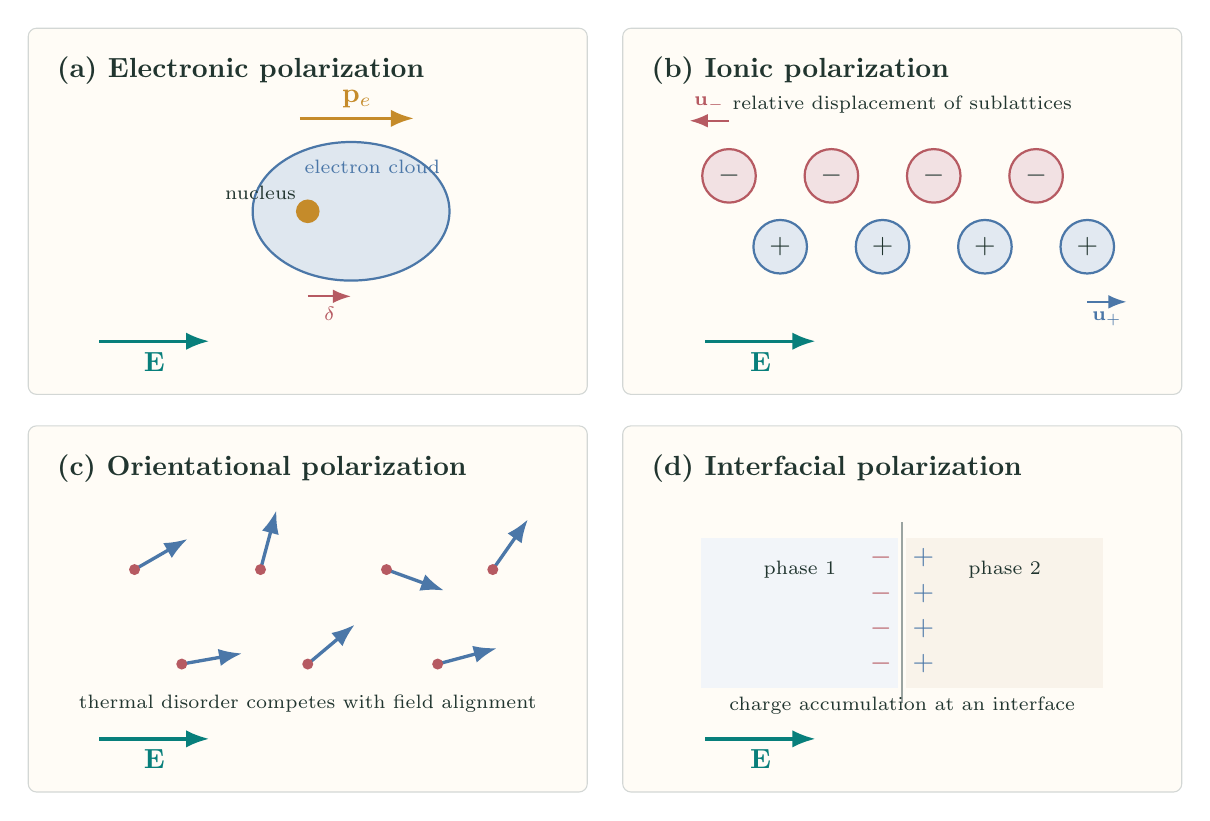
\begin{tikzpicture}[font=\sffamily, text=ink, >=Latex, panel/.style={draw=ink!20, rounded corners=3pt, fill=paper, minimum width=7.1cm, minimum height=4.65cm}]
  \node[panel] (a) at (0,0) {};
  \node[panel] (b) at (7.55,0) {};
  \node[panel] (c) at (0,-5.05) {};
  \node[panel] (d) at (7.55,-5.05) {};

  \node[anchor=north west, font=\bfseries] at ($(a.north west)+(0.25,-0.25)$) {(a) Electronic polarization};
  \draw[->, very thick, teal] (-2.65,-1.65) -- (-1.25,-1.65) node[midway,below] {$\mathbf E$};
  \fill[blue!18] (0.55,0) ellipse (1.25 and 0.88);
  \draw[blue, thick] (0.55,0) ellipse (1.25 and 0.88);
  \node[blue, font=\scriptsize] at (0.82,0.57) {electron cloud};
  \fill[gold] (0,0) circle (0.15) node[above left=1pt, font=\scriptsize, text=ink] {nucleus};
  \draw[->, thick, rose] (0,-1.08) -- (0.55,-1.08) node[midway,below, font=\scriptsize] {$\delta$};
  \draw[->, very thick, gold] (-0.1,1.18) -- (1.35,1.18) node[midway,above] {$\mathbf p_e$};

  \node[anchor=north west, font=\bfseries] at ($(b.north west)+(0.25,-0.25)$) {(b) Ionic polarization};
  \draw[->, very thick, teal] (5.05,-1.65) -- (6.45,-1.65) node[midway,below] {$\mathbf E$};
  \foreach \x in {5.35,6.65,7.95,9.25}{
    \fill[rose!18] (\x,0.45) circle (0.34); \draw[rose,thick] (\x,0.45) circle (0.34); \node at (\x,0.45) {$-$};
    \fill[blue!16] (\x+0.65,-0.45) circle (0.34); \draw[blue,thick] (\x+0.65,-0.45) circle (0.34); \node at (\x+0.65,-0.45) {$+$};
  }
  \draw[->,thick,rose] (5.35,1.15)--(4.85,1.15) node[midway,above,font=\scriptsize] {$\mathbf u_-$};
  \draw[->,thick,blue] (9.90,-1.15)--(10.40,-1.15) node[midway,below,font=\scriptsize] {$\mathbf u_+$};
  \node[font=\scriptsize] at (7.55,1.35) {relative displacement of sublattices};

  \node[anchor=north west, font=\bfseries] at ($(c.north west)+(0.25,-0.25)$) {(c) Orientational polarization};
  \draw[->, very thick, teal] (-2.65,-6.70) -- (-1.25,-6.70) node[midway,below] {$\mathbf E$};
  \foreach \x/\y/\ang in {-2.2/-4.55/30,-0.6/-4.55/75,1.0/-4.55/-20,2.35/-4.55/55,-1.6/-5.75/10,0/-5.75/40,1.65/-5.75/15}{
    \draw[very thick,blue,->] (\x,\y) -- ++(\ang:0.78);
    \fill[rose] (\x,\y) circle (0.07);
  }
  \node[font=\scriptsize, align=center] at (0,-6.25) {thermal disorder competes with field alignment};

  \node[anchor=north west, font=\bfseries] at ($(d.north west)+(0.25,-0.25)$) {(d) Interfacial polarization};
  \draw[->, very thick, teal] (5.05,-6.70) -- (6.45,-6.70) node[midway,below] {$\mathbf E$};
  \fill[blue!7] (5.0,-6.05) rectangle (7.5,-4.15);
  \fill[gold!10] (7.6,-6.05) rectangle (10.1,-4.15);
  \draw[ink!45,thick] (7.55,-6.25)--(7.55,-3.95);
  \foreach \y in {-5.75,-5.3,-4.85,-4.4}{
    \node[rose] at (7.28,\y) {$-$};
    \node[blue] at (7.82,\y) {$+$};
  }
  \node[font=\scriptsize] at (6.25,-4.55) {phase 1};
  \node[font=\scriptsize] at (8.85,-4.55) {phase 2};
  \node[font=\scriptsize, align=center] at (7.55,-6.28) {charge accumulation at an interface};
\end{tikzpicture}
\end{document}
